\chapter{Transformation de Laplace}
\section{Définition}
Soit $f : \mathbb{R} \to \mathbb{C}$ une application telle que~:
\begin{itemize}
\item $\forall t < 0, \, f(t) = 0$. ($f$ est dite \textit{causale}) 
\item $f$ est intégrable sur tout compact de $\mathbb{R}$.
\item Il existe un réel $x$ tel que l'intégrale~:
\[
\int_{\mathbb{R}^+}e^{-xt} f(t) dt
\]
soit convergente.
\end{itemize}

\begin{fdefn}
Soit $f$ une application vérifiant les conditions précédentes. La
transformée de Laplace de $f$ est l'application $\mathcal{L}(f) : \Omega \subset \mathbb{C} \to
\mathbb{C}$ définie par~:
\[
\mathcal{L}(f)(p) = \int_0^{+\infty}e^{-pt} f(t) dt
\]
$\Omega$ étant l'ensemble des $p$ pour lesquels l'intégrale précédente
est définie.
\end{fdefn}

\begin{fprop}
Si la transformation de Laplace de $f$ est définie pour $p_0$, elle
est également définie pour tout $p$ tel que $\Re(p) > \Re(p_0)$.
\end{fprop} 

La borne inférieure de l'ensemble des $x \in \R$ pour lesquels l'intégrale de
Laplace est convergente pour $\Re(p) = x$ est appelée abscisse de
convergence de la transformation de Laplace. 

On définira de même l'abscisse de convergence absolue, celle de $\vert f \vert$, qui est
supérieure ou égale à l'abscisse de convergence. On remarquera que
chacune de ces bornes peut être $-\infty$.

\begin{fprop}
Soit $p_0$ un complexe tel que la transformée de Laplace $\mathcal{L}(f)(p_0)$ de
$f$ soit définie. Soit $C_{\alpha, p_0}$ l'ensemble des complexes de
la forme $p_0 + r e^{i \theta}$ avec $r \in \mathbb{R}^+$ et $\theta
\in [-\alpha, \alpha]$. L'intégrale de Laplace est uniformément
convergente dans $C_{\alpha, p_0}$ si $\alpha \in ]0, \frac{\pi}{2}[$.
\end{fprop}

\begin{proof}
Soit $\epsilon > 0$ et soit $T > 0$ tel que pour tout $t > T$~:
\[
\lvert \int_T^t e^{-p_0 u}f(u) du \rvert  < \epsilon.
\]
On note $g(t) = \int_T^t e^{-p_0 u}f(u) du$.
Posons $p = p_0 + h$ pour $p \in C_{\alpha, p_0}$ et $h = r e^{i
\theta}$. On a~:
\[
\int_T^t e^{-p u}f(u) du = \int_T^t e^{-hu}g^\prime(u) du.
\]
Une intégration par parties conduit à~:
\[
\int_T^t e^{-hu}g^\prime(u) dt = e^{-ht}g(t) + h \int_T^t e^{-hu}g(u) du.
\]
Pour $t > T$ le premier terme est inférieur en module à $\epsilon$, alors que le
second est borné en module par~:
\[
r \epsilon \int_T^{+\infty} e^{-r u \cos(\alpha)} d u =
\frac{\epsilon}{\cos(\alpha)}.
\]
\end{proof}
La transformation de Laplace est holomorphe dans son domaine de
convergence comme le montre la proposition suivante.

\begin{fprop}
Soit $f$ continue sur $\mathbb{R}^+$ et soit $s$ l'abscisse de
convergence de sa transformée de Laplace $F$. Alors $F$ est
holomorphe dans le demi-plan complexe formé des points de partie
réelle strictement supérieure à $s$.
\end{fprop}

\begin{proof}
Soit $p = x+iy$ avec $x > s$. Soit $p_0 = x_0 + i y$ un point tel
que $s < x_0 < x$. Pour tout $\alpha \in ]0, \frac{\pi}{2}[$, le point
$p$ appartient à $C_{\alpha, p_0}$ et l'intégrale définissant $F$
est uniformément convergente dans $C_{\alpha, p_0}$. De plus,
l'application~:
$
p \mapsto e^{-pt} f(t)
$
est indéfiniment dérivable sur $C_{\alpha, p_0}$ et $t > 0$. On en
déduit alors (dérivation sous le signe somme) que $F(p)$ est
holomorphe dans $C_{\alpha, p_0}$ et que~:
\[
F^{(n)}(p) = (-1)^n \int_0^{+\infty} t^n f(t) e^{-pt} dt.
\] 
\end{proof}
\begin{rem}
La proposition reste vraie si $f$ est seulement continue par morceaux.
\end{rem}
\section{Propriétés}
La transformation de Laplace est de façon évidente linéaire. Son
intérêt principal vient de son comportement vis à vis de la
dérivation.

\begin{fprop}
Soit $f$ continue sur $\mathbb{R}^+$, dérivable. Si elle admet une
transformée de 
Laplace ainsi que sa dérivée, les deux transformées
sont liées par la relation~:
\[
\mathcal{L}(f^\prime)(p) = p \mathcal{L}(f)(p) - f(0^+)
\] 
avec $f(0^+) = \lim_{ t \to 0, \; t > 0} f(t)$
\end{fprop}

\begin{proof}
On a~:
\[
\mathcal{L}(f^\prime)(p) = \lim_{t\to + \infty} \int_0^Tf^\prime(t) e^{-pt} dt.
\]
Une intégration par parties montre que l'intégrale de droite vaut~:
\[
\left [
e^{-pt}f(t)
\right ]_0^T
+ p \int_0^T f(t) e^{-pt} dt.
\]
Qui montre la proposition par passage à la limite.
\end{proof}
Cette proposition s'étend par récurrence pour les dérivées d'ordre
quelconque~:
\[
\mathcal{L}(f^{(n)})(p) = p^n \mathcal{L}(f)(p) - p^{n-1} f(0)
- p^{n-2} f^\prime(0) - \dots f^{(n-1)}(0^+)).
\]
Il est possible de déterminer également la transformée de Laplace de
la primitive d'une application.

\begin{fprop}
Si $f$ admet une transformée de Laplace $F$ et si $\lim_{t \to 0^+}
\frac{f(t)}{t}$ existe, alors~:
\[
\mathcal{L} \left( \frac{f(t)}{t} \right) (p) = \int_p^{+\infty} F(u) du.
\]
\end{fprop} 

\begin{proof}
\[
\int_p^Z F(u) du = \int_p^Z \int_0^{+\infty} e^{-ut}
f(t) dt du
\]
comme l'intégrale de Laplace est uniformément convergente dans un
secteur angulaire, on peut intervertir l'ordre de intégrations et
l'intégrale devient~:
\[
\int_0^{+\infty} e^{-pt} \frac{f(t)}{t} dt - \int_0^{+\infty} e^{-Zt} \frac{f(t)}{t} dt
\] 
La conclusion s'obtient en faisant tendre $Z$ vers l'infini en module.
\end{proof}

\begin{fprop}
Soit $f$ de transformée de Laplace $F$ et soit $s$ l'abscisse de
convergence de cette transformée. Alors l'application~:
\[
\int_0^t f(u) du
\]
admet pour transformée de Laplace $\frac{F(p)}{p}$ et son abscisse de
convergence est strictement supérieure à $\sup(0, s)$.
\end{fprop}

Cette proposition se montre de façon similaire à la précédente.
\begin{fprop}
Soit $f$ admettant une transformée de Laplace $F$ d'abscisse de
convergence $s$. Soit $a \in \mathbb{C}$. Alors l'application
$e^{at}f(t)$ admet pour transformée de Laplace $F(p-a)$, son abscisse
de convergence étant $s + \Re(a)$.
\end{fprop}
\begin{fprop}
Soit $f$ admettant $F$ pour transformée de Laplace. Soit $a \in
\mathbb{R}$. Alors
l'application $g$ telle que $g(t) = 0$ si $t < a$ et $g(t) = f(t-a)$
sinon admet pour transforméee de Laplace $e^{-ap}F(p)$.
\end{fprop}
Ces deux propositions se montrent de manière immédiate.
On peut calculer facilement à partir de ceci la transformée de Laplace
d'une application périodique. Soit $f_1$ une application à support
dans un intervalle réel $[0,T]$ et soit $f$ l'application définie par
périodisation de $f_1$ de période $T$. Si $f$ admet une transformée de
Laplace et si $F_1$ est la transformée de Laplace de $f_1$, alors~:
\[
\mathcal{L}(f)(p) = \frac{F_1(p)}{1-e^{-pT}}.
\]
Ce résultat s'obtient en écrivant $f$ sous la forme d'une somme de
termes de la forme $f_1(t-k T)$ avec $k \in \mathbb{N}$ et en faisant
apparaître une série géométrique.
On a enfin une proposition relative aux changements d'échelle.
\begin{fprop}
Si $f$ admet pour transformée de Laplace $F$ alors, pour $\lambda \in
\mathbb{R^*}$, l'application $f\left( t/\lambda \right)$ admet pour transformée de
Laplace $\lambda F(\lambda p).$
\end{fprop}
\section{Inversion}

\begin{fprop}(Théorème de la valeur finale)
Soit $f$ continue de transformée de Laplace $F$. Si l'abscisse de convergence
$s$ est négative et si $\lim_{t \to +\infty}f(t)$ existe, alors~:
\[
\lim_{p \to 0^+} p F(p) = \lim_{t \to +\infty} f(t).
\]
\end{fprop}

\begin{proof}
Soit $l = \lim_{t \to +\infty} f(t)$. 
\begin{align*}
pF(p) - l & = p \int_0^{+\infty} e^{-pt}f(t) dt - l \\
&= p \int_0^T  e^{-pt}f(t) dt + p  \int_T^{+\infty}e^{-pt}(f(t) -l) dt
\\ &+ l \left (
p \int_T^{+\infty} e^{-pt}dt -1
\right )
\end{align*}
Le premier terme est majoré en module par~:
\[
|p| T M_T
\]
avec $M_T$ borne $\sup$ de $|f|$ sur $[0,T]$.
Le second terme se majore uniformément par définition de la limite de
$f$ en $+\infty$ et la convergence uniforme de l'intégrale. Enfin, le
troisième terme tend vers 0 pour $|p|\to 0^+$, ce qui montre la proposition.
\end{proof}

\begin{fprop}(Théorème de la valeur initiale)
Soit $f$ dérivable, de transforméee de Laplace $F$ et telle que sa
dérivée soit également transformable. Alors~:
\[
\lim_{|p|\to +\infty} p F(p) = f(0^+)
\]
\end{fprop}

\begin{proof}
On a~:
\[
\lim_{|p| \to +\infty} \mathcal{L}(f^\prime)(p) = 0
\]
et $\mathcal{L}(f^\prime)(p) = p F(p) - f(0^+)$.
\end{proof}

\begin{fprop}
Soit $f$ définie par une série entiére convergente $\sum_{n \in
\mathbb{N}} a_n z^n$ de rayon de convergence infini. Alors elle
est transformable et sa transformée s'obtient en transformant terme à terme.
\end{fprop}

\begin{fdefn}
Soit $[a,b]$ un intervalle de $\mathbb{R}$. Soit $f : [a,b] \to \mathbb{R} (\mbox{ resp. } \mathbb{C})$. On dira
que $f$ est à variation bornée si~:
\[
\sup \{ \sum_{i=0\dots N-1} |f(t_{i+1}) - f(t_i)|, \, a = t_0 < t_1, \dots < t_N = b, \, N \in \mathbb{N} \} < + \infty
\]
\end{fdefn}
La définition précédente s'étend immédiatement au cas des intervalles semi-infinis ou infinis.
La proposition suivante est très classique~:
\begin{fprop}(Lemme de Dirichlet)
Soit $f$ à variation bornée sur un intervalle $[0,a]$. On a~:
\[
\lim_{b \to +\infty} \int_{[0,a]} f(x) \frac{\sin bx}{x} d \lambda(x) =
f(0^+) \lim_{T \to +\infty} \int_{[0,T]} \frac{\sin x}{x} d \lambda(x).
\]
\end{fprop}

\begin{fthm}
Soit $F$ la transformée de Laplace d'une application à variation bornée $f$, l'abscisse
de convergence étant $s$. En tout point de continuité $t$ de $f$, on a~:
\[
f(t) = \frac{1}{i 2 \pi} \lim_{b \to + \infty} \int_{a-ib}^{a+ib}
e^{pt} F(p) dp
\]
avec $a > s$.
\end{fthm}

\begin{proof}
Formons~:
\[
f_b(t) = \frac{1}{i 2 \pi}  \int_{a-ib}^{a+ib} e^{pt} \int_0^{\infty}
e^{-pu} f(u) du dp.
\]
La convergence de l'intégrale étant uniforme, on peut écrire, après
interversion des intégrales~:
\[
f_b(t) = \frac{1}{\pi} e^{at} \int_{-t}^{+\infty} f(u+t)e^{-a(u+t)}
\frac{\sin (b u)}{u} du.
\]
Comme par ailleurs $f(t) = 0$ pour $t < 0$, on a~:
\[
f_b(t) = \frac{1}{\pi} e^{at} \int_{-\infty}^{+\infty} f(u+t)e^{-a(u+t)}
\frac{\sin (b u)}{u} du.
\]
Soit encore~:
\[
f_b(t) = \frac{1}{\pi} e^{at} \int_{0}^{+\infty} \left (
f(u+t)e^{-a(u+t)} + f(t-u)e^{-a(t-u)}
\right )
\frac{\sin (b u)}{u} du.
\]
En utilisant~:
\[
\int_0^{+\infty} \frac{\sin (b u)}{u} du = \frac{\pi}{2}
\]
on obtient~:
\[
f_b(t) = f(t)  + \frac{1}{\pi} e^{at} \int_{0}^{+\infty} \left (
f(u+t)e^{-a(u+t)} + f(t-u)e^{-a(t-u)} - 2 f(t)e^{-at}
\right )
\frac{\sin (b u)}{u} du.
\]
Le résultat s'obtient alors en faisant tendre $b$ vers $+\infty$ et en utilisant le lemme de Dirichlet.
\end{proof} 
Il existe une forme réciproque de ce théorème~:

\begin{fthm}(Formule d'inversion de Mellin-Fourier)
Soit une application $F$ analytique dans un demi-plan $\Re(p) > s_0$,
tendant vers 0 pour $|p| \to +\infty$ dans tout demi-plan $\Re(p) > s
> s_0$. Si l'intégrale~:
\[
\int_{s-i \infty}^{s+i \infty} F(p) dp
\]
converge absolument pour $s > s_0$, alors $F$ est la transformée de
Laplace de l'application $f$ définie par~:
\[
f(t) = \frac{1}{i 2 \pi} \int_{s-i \infty}^{s+i \infty} F(p) dp.
\]
On dira que $f$ est l'original de $F.$
\end{fthm}

Le contour de la figure \ref{fig:contour_laplace} (contour de Bromwich-Wagner) est fréquemment employé pour calculer l'original d'une transformée de Laplace par la formule de Mellin-Fourier.
\begin{figure}
    \centering
    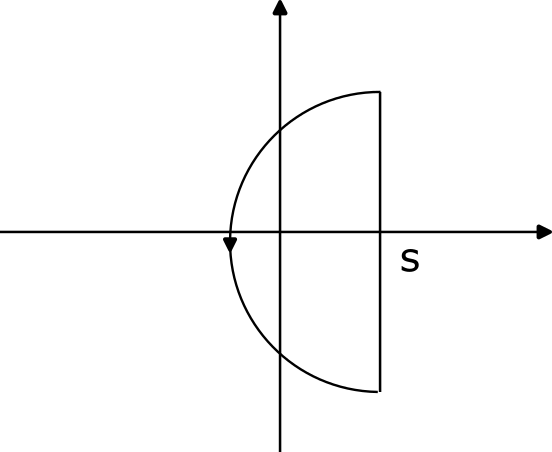
\includegraphics[scale=0.8]{images/contour_laplace.png}
    \caption{Contour de Bromwich-Wagner pour la transformée de Laplace inverse.}
    \label{fig:contour_laplace}
\end{figure}
En pratique, on inversera le plus souvent une transformée de Laplace en utilisant des tables, ou un logiciel de calcul formel comme \texttt{Mathematica}.

\begin{exercice}
On veut déterminer l'original de l'application~:
\[
F : p \to \frac{1}{1+p^3}
\]
\begin{itemize}
\item Calculer, en précisant l'abscisse de convergence, la transformée de Laplace de l'application:
\[
f \colon t \mapsto \begin{cases}
    0 & t< 0 \\
    e^{-at} & t \geq 0, a \in \C
\end{cases}
\]
\item Décomposer $F$ en éléments simples et en déduire son original $f.$
\item Retrouver ce résultat par la formule d'inversion de Mellin-Fourier.
\end{itemize}
\end{exercice}

\newpage 
\subsection*{Un peu d'histoire \dots}

\begin{minipage}{0.2\linewidth}
\begin{center}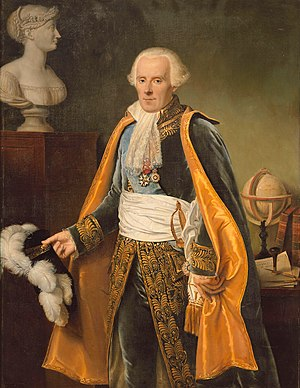
\includegraphics[width=2.9cm]{images/Laplace.jpeg}\end{center}
\end{minipage}
\begin{minipage}{0.8 \linewidth}
\small{\paragraph*{Pierre-Simon, marquis de Laplace :} né le 23 mars 1749 à Beaumont-en-Auge (Calvados) et mort le 5 mars 1827 à Paris, est un mathématicien, astronome, physicien et homme politique français. Il utilisa une notion proche de la transformation portant son nom en 1774 dans le cadre de ses travaux sur la théorie des probabilités. Pour Laplace, la nature est l'essence de la découverte scientifique et les mathématiques ne sont qu'un instrument pour la décrire. Laplace est avant tout un théoricien de l'astronomie, mais sa passion pour cette discipline est le prétexte à de nombreuses études mathématiques, en particulier dans le domaine des équations différentielles et en théorie des probabilités. 

Peu intéressé par les idées révolutionnaires, il reste politiquement neutre. Napoléon entretient de bons rapports avec lui et le nomme Ministre de l'Intérieur en 1799, poste qu'il n'occupera qu'un mois. Plus tard, Napoléon lui reprochant de ne pas citer Dieu dans son \textit{Traité de Mécanique Céleste} (1812), Laplace lui répond : "Je n'ai pas besoin de cette hypothèse".  
}
\end{minipage}

\vfill